\chapter{Interaction Region Local Coupling Correction in the LHC} % Main chapter title
\label{chapter:IR_Local_Coupling} % For referencing the chapter elsewhere, use \cref{chapter:IR_Local_Coupling}

\todo{Some paragraph before the first section.}

%----------------------------------------------------------------------------------------

\section{Local Betatron Coupling in the LHC Interaction Regions}
\label{section:local_ir_coupling}

In the LHC, corrections of local IR linear coupling are of importance to keep a good control of beam sizes at the IPs and hence the luminosity performance, as well as to prevent a significant impact on the beam dynamics.

In \cref{equation:coupling_rdts_from_skew_quads} the contribution of elements to the linear coupling RDTs is given, where contributing elements are typically skew quadrupoles and solenoids.
The amplitude of the contribution is dominated by the integrated strength of the magnet \(k L\) as well as the \(\sqrt{\beta_x \beta_y}\) term at the location of the magnet.
Given that a tilted quadrupole interacts with the beam as a straight quadrupole with an additional skew quadrupolar component, once can see from \cref{figure:ir5_and_around} that any tilt in the triplet quadrupoles would generate a massive contribution to the coupling RDTs due to the very high \(\beta\)-functions in these magnets.

\Cref{figure:triplet_tilts_to_rdts} shows the coupling RDTs' amplitudes from tilts in triplet quadrupoles, with the \(\beta^{\ast} =\)~\qty{30}{\centi\meter} \num{2022} optics.
In this MAD-X simulation triplets around IP\num{1} were assigned random tilts within \(\pm\)~\qty{1.5}{\milli\radian}, and these were the only contribution to coupling in the machine.
Nevertheless, this contribution amounted to a \(\abs{C^{-}}\) of \num{3.84e-2}, too high for machine operation.

\begin{figure}[!htb]
    \centering
    \includegraphics*[width=0.99\columnwidth]{Figures/IR_Coupling_Correction/triplet_tilts_to_rdts.pdf}
    \caption{Amplitudes of the coupling RDTs (bottom) \(f_{1001}\) (\textcolor{mplblue}{blue}) and \(f_{1010}\) (\textcolor{mplorange}{orange}) from tilts in the triplet quadrupoles around IP\num{1}. The top plot shows the magnets' powering while the middle plot shows the assigned tilts in each element.}
    \label{figure:triplet_tilts_to_rdts}
\end{figure}

As a consequence, the IR contribution - mainly the triplets - to global coupling needs to be compensated.
For this, in the LHC the local coupling correction is done by measuring the RDTs in the vicinity of the IP and using the MQSX skew quadrupole correctors introduced in \cref{subsection:lhc_eirs} and showcased in \cref{figure:ir5_and_around,figure:lhc_ir_corrector_layout} for correction.
The corrections are determined with the Segment-by-Segment technique described in \cref{subsection:correction_principles}, and try to cancel the triplets' contribution as well as possible.
Though this compensation is rarely perfect, the residual contribution is usually small enough to be handled by the skew quadrupole correctors present in the LHC arcs (see \cref{subsection:lhc_arcs}).
This correction is essential in order to reach low \(\beta^{\ast}\) with good optics control: at \(\beta^{*}=\) \qty{30}{\centi\meter} the local errors compensated in Run~\num{2}~\cite{CERN:Persson:LHCOpticsCorrectionsEvian2019} would contribute to the \(\abs{C^{-}}\) by the amount of \num{0.33}, too high for the arc correctors to handle.

During the late \num{2018} ion run in the LHC Run~\num{2}, it was observed that while global coupling was well corrected, a local coupling bump in the IR\num{2} had a significant impact on collisions and led to a reduction of the luminosity at the affected IP by up to \qty{50}{\percent}~\cite{IPAC:Jowett:LHC_2018_Heavy_Ion_Run, IPAC:Tomas:Run2_Experience_View_LHC_HLLHC, CERN:Persson:LHCOpticsCorrectionsEvian2019}.
Investigations revealed that a coupling bump around IP\num{2} led to a strong increase in beam size and a drop in collisions.
Importantly, the incident highlighted that no method existed to correct for the coupling specifically at the IP location.

\Cref{figure:lhc_vs_hllhc_beam_size_and_lumi_growths} shows the expected beam size growth and luminosity decrease from various strengths of such a local coupling bump at IP\num{1} or IP\num{5}, for the LHC at \(\beta^{*}=\) \qty{30}{\centi\meter} and for the HL-LHC at \(\beta^{*}=\) \qty{15}{\centi\meter}.
These results highlight the necessity of a proper handling of local coupling for the Run~\num{3}, as well as for the HL-LHC where it should be about a factor \num{4} more accurate.

\begin{figure}[!htb]
    \centering
    \includegraphics*[width=0.99\columnwidth]{Figures/IR_Coupling_Correction/lhc_vs_hllhc_combined.pdf}
    \caption{Relative values of the RMS beam size at IP\num{1} (\textcolor{mplblue}{blue}) as well as luminosity (\textcolor{mplorange}{orange}) for different strengths of a local coupling bump around the IP made with skew quadrupoles, for the LHC (filled) and HL-LHC v1.5 (dashed) collision optics.}% Beam sizes are calculated according to \cref{equation:lebedev_beam_size} and luminosities according to \cref{equation:luminosity_double_beams}. In the case of the HL-LHC, the relative beam size increase and subsequent luminosity loss are greater due to the much larger \(\beta\)-functions in the triplet.}
    \label{figure:lhc_vs_hllhc_beam_size_and_lumi_growths}
\end{figure}

In the studies presented in this thesis, various calculations rely heavily on the Ripken parameters mentioned in \cref{subsection:parametrization_of_betatron_coupling}.
For instance, beam sizes are calculated from the \(\beta_{kj}\) terms according to~\cite{IOP:Lebedev:Betatron_Motion_Coupling}:

\begin{equation}
    \langle z \rangle = \sqrt{\varepsilon_1 \beta_{1z} + \varepsilon_2 \beta_{2z}}, \quad z \in\{x, y\} ,
    \label{equation:lebedev_beam_size}
\end{equation}
where \(\varepsilon_1\) and \(\varepsilon_2\) are the horizontal and vertical emittances, respectively.

The validity of this calculation has been verified in simulations by comparing its results to those obtained from other means.
\Cref{figure:lebedev_vs_tracking} shows the relative deviation between computed beam sizes at IP\num{5}, calculated either according to \cref{equation:lebedev_beam_size} or from tracking a particle distribution, under various strengths of local coupling.
In all cases the relative deviation is below \qty{0.25}{\percent}.

\begin{figure}[!htb]
    \centering
    \includegraphics*[width=0.99\columnwidth]{Figures/IR_Coupling_Correction/lebedev_vs_tracking.pdf}
    \caption{Relative deviation between beam sizes calculated from Ripken parameters according to \cref{equation:lebedev_beam_size} and from tracking a particle distribution, at an IP affected by coupling for the horizontal (\textcolor{mplblue}{blue}) and vertical (\textcolor{mplorange}{orange}) planes.}
    \label{figure:lebedev_vs_tracking}
\end{figure}

At the LHC IPs with round beams, as is the case in Run~\num{3}, the effect of the beam's tilt induced by linear coupling is negligible and its impact manifests as an increase in the beam size, as was the case at IP\num{2} in \num{2018}.
\Cref{figure:ip_ellipses_from_coupling} shows a reconstruction of transverse beam sizes at IP\num{1} (similar for IP\num{5}) under various strengths of a local coupling bump.
While the beam ellipses show a \(\gg\) \qty{99}{\percent} overlap indicating a negligible tilt effect, the beam size in the most affected case is about \qty{250}{\percent} of the uncoupled case.

\begin{figure}[!htb]
    \centering
    \includegraphics*[width=0.75\columnwidth]{Figures/IR_Coupling_Correction/ellipses_various_coupling_bumps.pdf}
    \caption{Transverse beam sizes at IP\num{5} at \qty{6.8}{\tera\electronvolt} and \(\beta^{\ast}=\)~\qty{30}{\centi\meter} with normalized emittances \(\varepsilon_x = \varepsilon_y =\)~\qty{3.75}{\micro\meter} and for different strengths of a local coupling bump around the IP. The ellipses are reconstructed through the \(\sigma_{11}\), \(\sigma_{13}\) and \(\sigma_{33}\) terms of the sigma matrix, obtained from MAD-X.}
    \label{figure:ip_ellipses_from_coupling}
\end{figure}

Instantaneous luminosities calculated for~\cref{figure:lhc_vs_hllhc_beam_size_and_lumi_growths}, in the absence of crossing angles, are done so according to~\cite{CERN:Herr:Concept_Luminosity}:

\begin{equation}
    \mathcal{L} = \frac{N_1 N_2 f_{rev} N_b}{2 \pi \sqrt{\left( \sigma_{x, 1}^2 + \sigma_{x, 2}^2 \right)} \sqrt{\left( \sigma_{y, 1}^2 + \sigma_{y, 2}^2 \right)}} ,
    \label{equation:luminosity_double_beams}
\end{equation}
where \(N_{n}\) is the number of protons per bunch in beam \(n\), \(f_{rev}\) the revolution frequency of particles, \(N_b\) the number of bunches per beam and \(\sigma_{z, n}\) is the size at the IP of beam \(n\) in the transverse plane \(z\), calculated according to \cref{equation:lebedev_beam_size}.

\todo{What else to add here? I should say a bit that we want to look into getting coupling control at the IP, for the reasons. This transitions into the next section.}

\section{Current Correction Methods and Their Limitations}
\label{section:current_correction_methods_and_their_limitations}

\textbf{Things to include in here:}
\begin{itemize}
    \item Say that just from RDTs there isn't really a way to know, with \cref{figure:guess_rdts} as example
    \item Go over (see PRAB paper) an overview of IR Difficulties (phase advances suck, DFFT of x -jpx, no instruments, SbS errors)
    \item Emphasize that not only is SbS not great, it doesn't give us a way to optimize the coupling at the IP
    \item Mention that because correctors are single aperture, we need to find a correction compromise that works well for B1 and B2
    \item Mention K-Modulation (cite M. Hofer's paper)
    \item Mention the CRDTs but not much is visible (remake plot from study)
    \item Introduce the colinearity knob
\end{itemize}

In the LHC, a skew quadrupole corrector is installed on each side of colliding IPs, just before the third triplet quadrupole \(\mathrm{Q3}\) on the side of the IP.
Due to their location, these correctors are single aperture magnets meaning that both beams are passing through a single cavity, and feel the same magnetic field.
As the triplet quadrupoles - also single aperture magnets - are expected to be most of the contribution to local coupling, the local error to be corrected should be the same for both beams and such an arrangement of correctors is manageable.

Say that looking at RDTs is just not straightforward, and give example with plot below. Can you guess who's better? I forgot already.
\begin{figure}
    \centering
    \includegraphics*[width=0.99\linewidth]{Figures/IR_Coupling_Correction/similar_rdts_different_ip1_lumi.pdf}
    \caption{Similarly looking coupling RDTs from two measurements (top and bottom) in the LHC \num{2022} commissioning. One scenario leads to a \qty{20}{\percent} luminosity decrease at IP\num{1} compared to the other. Can you tell which is which?}
    \label{figure:guess_rdts}
\end{figure}

\begin{table}[!hbt]
    \centering
    \begin{tblr}{colspec={ccccc}}
        \hline
        \textbf{Magnet} & \textbf{K\(_{1S}\) [m\(^{-2}\)]}    \\
        \hline
        MQSX.3R[IP] \(\rightarrow K_{1S}\)  &  \num{1E-4}   \\
        MQSX.3L[IP] \(\rightarrow K_{1S}\)  &  \num{-1E-4}  \\
        \hline
    \end{tblr}
    \caption{Definition of one unit of the colinearity knob, a powering setting of the IR skew quadrupole correctors.}
    \label{table:colin_knob}
\end{table}

\begin{figure}
    \centering
    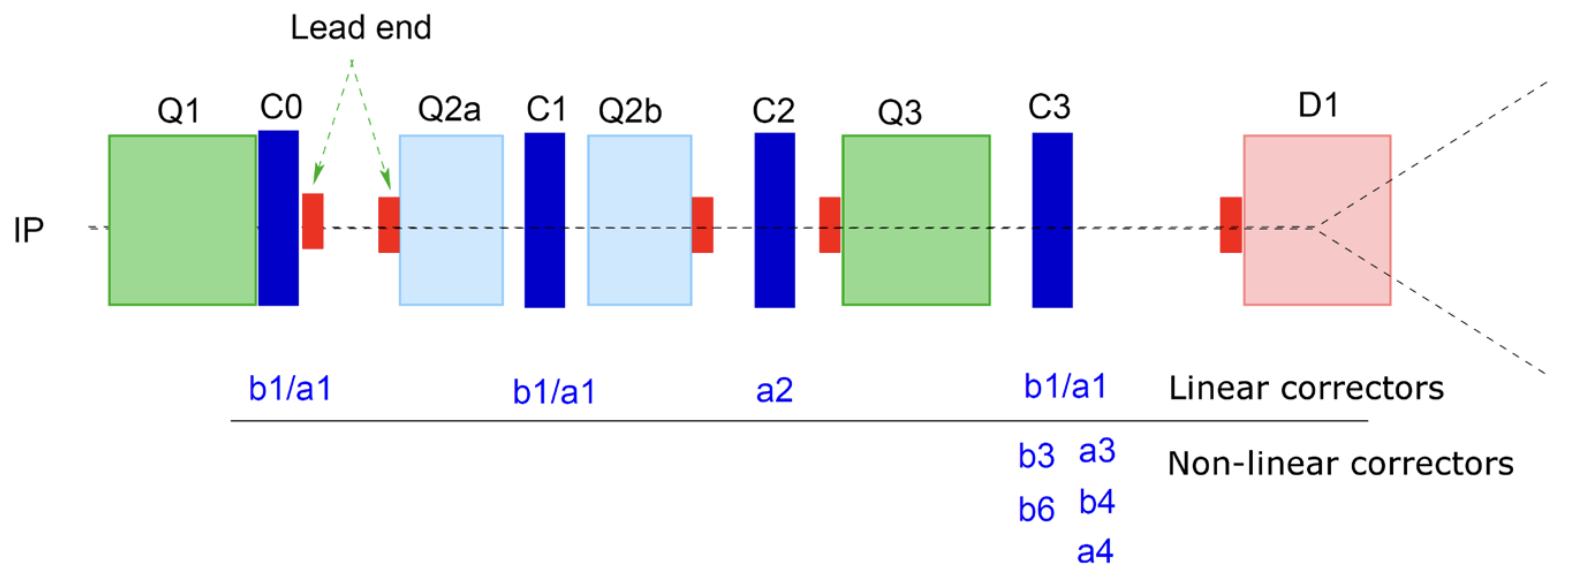
\includegraphics[width=0.9\linewidth]{Figures/IR_Coupling_Correction/corrector_package.png}
    \caption{Layout of the triplet magnets and the linear and nonlinear correctors in the LHC experimental insertions~\cite{CERN:Bruning:Dynap_Studies}, showing common aperture magnets. The Q\num{1}, Q\num{2}a/b and Q\num{3} are triplet quadrupoles while the C\num{0}, C\num{1}, C\num{2} and C\num{3} are corrector packages with the field order indicated below. D\num{1} is the separation dipole, diverging Beam \num{1} and Beam \num{2} to their respective beam lines. The skew quadrupole correctors correspond to order a\num{2} and are located in the C\num{2} package.}
    \label{figure:lhc_corrector_layout}
\end{figure}

\todo{Here include also the stuff that didn't work (CRDTs, k-modulation, etc.)}

\section{Rigid Waist Shift for Local Coupling Correction}
\label{section:rigid_waist_shift_for_local_coupling_correction}

\subsection{Concept and Simulations}

\begin{figure}
    \centering
    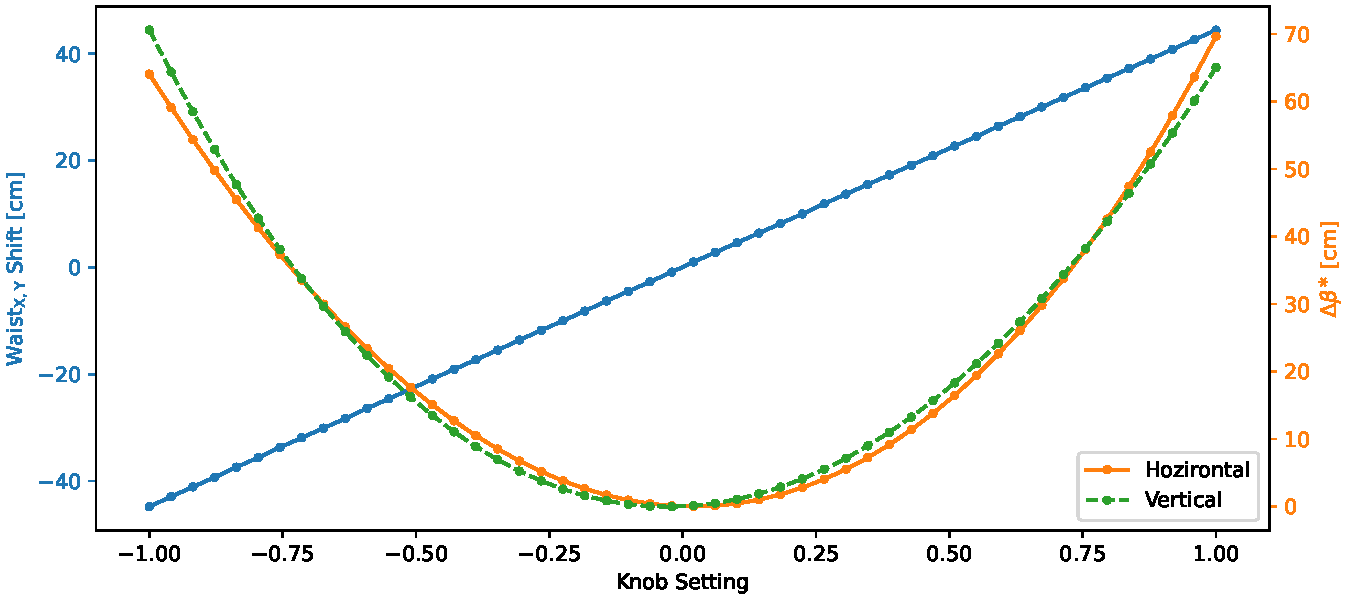
\includegraphics[width=0.9\textwidth]{Figures/IR_Coupling_Correction/rigid_waist_shift_effect_combined.pdf}
    \caption{Simulated effect of the designed rigid waist shift knob on the \(\beta^{\ast} =\) \qty{30}{\centi\metre} collision optics. The \textcolor{mplblue}{blue} line represents the waist displacement from the design location and is almost completely linear with the knob setting. The \textcolor{mplorange}{orange} and \textcolor{mplgreen}{green} lines represent the horizontal and vertical \(\beta\)-functions change at the IP point itself as the waist is displaced, respectively. The minima of the parabolas are not found at the zero knob setting as the design optics include a very small waist.}
    \label{figure:rigid_waist_shift_knob_effect1}
\end{figure}

\begin{figure}[!htb]
    \centering
    \includegraphics*[width=\columnwidth]{Figures/IR_Coupling_Correction/waist_shift_leaks_rdts.pdf}
    \caption{Linear coupling RDTs in the vicinity of IP\num{1} under a coupling bump, with (\textcolor{mplr}{red}) and without (\textcolor{mplb}{blue}) an RWS. The vertical \textcolor{mqsx_green}{green} lines represent the positions of the skew quadrupoles correctors (MQSX.\num{3}[RL]\num{1}) used to implement the coupling bump. A colinearity knob setting of \num{10} and a rigidity waist shift knob setting of \num{1} were used, which results in a \qty{0.5}{\percent} change in the triplet powering knob and a \qty{43.5}{\centi\meter} shift of the beam waists.}
    \label{figure:rdt_leak}
\end{figure}

\begin{figure}[!htb]
    \centering
    \includegraphics*[width=0.99\columnwidth]{Figures/IR_Coupling_Correction/colin_knob_vs_waist_shift.pdf}
    \caption{Impact of the colinearity knob on the global \(\abs{C^{-}}\), calculated according to \cref{equation:deltaqmin_from_f1001}, with and without applying an RWS.}
    \label{figure:knob_to_cminus_with_waist}
\end{figure}

\Cref{figure:cminus_colin_vs_tilt_with_waist} shows the values of the resulting \(\abs{C^{-}}\) across the parameter space when an RWS is applied.

\begin{figure}[!htb]
    \centering
    \includegraphics*[width=0.99\columnwidth]{Figures/IR_Coupling_Correction/cminus_colin_tilt_compensation_with_waist.pdf}
    \caption{Resulting \(\abs{C^{-}}\) (\cref{equation:deltaqmin_from_f1001}) for various combinations of tilt error and colinearity knob settings, when applying an RWS.}
    \label{figure:cminus_colin_vs_tilt_with_waist}
\end{figure}

\Cref{figure:beam_size_colin_vs_tilt_no_waist} shows the resulting beam size increase as a ratio to the nominal beam size across the same parameter space, highlighting that minimization of the growth is possible though a wrong setting would enhance the phenomenon.

\begin{figure}[!htb]
    \centering
    \includegraphics*[width=0.99\columnwidth]{Figures/IR_Coupling_Correction/ip_beam_size_growth_colin_tilt_compensation_no_waist.pdf}
    \caption{Resulting beam size (\cref{equation:lebedev_beam_size}) increase for identical settings of tilt error and colinearity knob settings as \cref{figure:cminus_colin_vs_tilt_with_waist}, but without an RWS.}
    \label{figure:beam_size_colin_vs_tilt_no_waist}
\end{figure}

\subsection{Determining Corrections}

Blah.

\subsubsection*{Rigid Waist Shift Procedure}

Bleh.

%----------------------------------------------------------------------------------------

\section{Experimental Results from the LHC \num{2022} Commissioning}
\label{section:rws_experimental_results}

Can refer to appendix \Cref{appendix:experimental_knobs} for the fills used.

\begin{table}[!htb]
    \centering
    \caption{Luminosity gains observed at the main experiments ATLAS and CMS from the method's suggested corrections.}
    \begin{tblr}{colspec={ccc}}
        \hline
        \SetCell[r=2,c=1]{m,c} \textbf{Experiment} & \SetCell[c=2]{c} \textbf{Luminosity Gain [\unit{\percent}]}                     \\
        \cline{2,3}                                &    \(\beta^{\ast} = \) \qty{30}{cm}    &    \(\beta^{\ast} = \) \qty{42}{cm}    \\
        \hline
        \textbf{ATLAS (IP\num{1})}                 &    \num{9.7}                           &     \num{5.2}                          \\
        \textbf{CMS (IP\num{5})}                   &    \num{3.5}                           &     \num{1.5}                          \\
        \hline
    \end{tblr}
    \label{table:rws_lumi_gains}
\end{table}

\section{Operation with Limited Correctors Availability}
\label{section:limited_correctors_availability}

Mitigation Options in Case of MQSX Failures
\todo{Uncomment text when I get here, take mostly the structure of the IPAC23 article and project update V. Go deeper in details (see commented out subsections).}

% \subsection{Lifetime Considerations of MQSX Elements}

% Explain that there is a real risk that some of our MQSX magnets die, especially the ones in IR1 (ATLAS).
% In this case, we will need a containment plan, as not only are they used for the but the local corrections they are a part of are a baseline for us to compute higher order terms corrections.

% \Cref{table:correctors_peak_dose} reproduced from slide 23~\cite{Evian21:Cerutti:TripletLifetime}:

% \begin{table}[!htb]
%     \centering
%     \caption{Expected total received dose of the corrector magnets located in the triplets for the main IRs. Table reproduced from~\cite{Evian21:Cerutti:TripletLifetime}. The entries marked with \asterisk assume an IR\num{1} polarity inversion in the middle of \num{2025}.}
%     \begin{tblr}{colspec={ccc}}
%         \hline
%         \SetCell[r=3,c=1]{m,c} \textbf{Magnets}             &  \SetCell[c=2]{c} \textbf{Peak Dose [\unit{\mega\gray}]}                                                                                     \\
%         \cline{2,3}                                         &  With ATLAS Variable (Fixed) Angle                        &    +\num{2025} (as \num{2023}/\num{2024})                                        \\
%         \cline{2,3}                                         &  After \qty{395}{\femto\barn^{-1}}                        &    After \qty{480}{\femto\barn^{-1}}                                             \\
%         \hline
%         \textcolor{red}{\textbf{MCBX\num{1} (IR\num{1})}}   &    \textcolor{red}{\num{8.5} (\num{8.5})}                 &     \textcolor{red}{\num{11} (\num{11}) $/$ \asterisk \num{10.5} (\num{10.5})}   \\
%         \textcolor{red}{\textbf{MCBX\num{1} (IR\num{5})}}   &    \num{6}                                                &     \textcolor{red}{\num{7.5}}                                                   \\
%         \textbf{MCBX\num{2} (IR\num{1})}                    &    \num{3.5} (\num{3.5})                                  &     \num{4} (\num{4}) $/$ \asterisk \num{4} (\num{4})                            \\
%         \textbf{MCBX\num{2} (IR\num{5})}                    &    \num{2}                                                &     \num{2.5}                                                                    \\
%         \textcolor{red}{\textbf{MQSX (IR\num{1})}}          &    \textcolor{red}{\num{7.5} (\num{7.5})}                 &     \textcolor{red}{\num{9} (\num{9}) $/$ \asterisk \num{9} (\num{9})}           \\
%         \textcolor{red}{\textbf{MQSX (IR\num{5})}}          &    \textcolor{red}{\num{8} (\num{8})}                     &     \textcolor{red}{\num{9.5} (\num{9.5})}                                       \\
%         \textbf{MCBX\num{3} (IR\num{1})}                    &    \num{5} (\num{5})                                      &     \num{6} (\num{6.5}) $/$ \asterisk \num{6} (\num{6})                          \\
%         \textbf{MCBX\num{3} (IR\num{5})}                    &    \num{3}                                                &     \num{3.5}                                                                    \\
%         \hline
%     \end{tblr}
%     \label{table:correctors_peak_dose}
% \end{table}

% \todo{Important quote from the end of the presentation:}
% "Assuming a limit of \qty{6}{\mega\gray} for the corrector magnets in the triplet, this is expected to be reached in the four \(\mathrm{MCBX.1}\) and four \MQSX by the end of \num{2024}."

% This means in simple terms that MQSX dying will drastically impact the LHC's operations, and potentially shut the machine down.

% \subsection{Tilt of Triplet Elements}

% Talk about what we want to do (tilt Q3 or Q2) to induce a skew component + simulation results.
% Found settings of the Q3 or Q2 that would negate the MQSX one determined in beam test / commissioning.
% Show some plots, and come up with the tilt values that would be needed to do the compensation.

% Also show we have a very minimal beta-beating from this.
% Show we have had a look at different optics (30cm and 1m betastar) and it works for both.

% \subsubsection*{Operational Constraints}

% The LHC systems are not meant for this, but for vertical alignment of these magnets!
% System relies on bellows: 2 pieds IP side and 1 pied other side for Q2 for instance.
% This means that inducing rotation is not only not the design purpose, but also imperfect (on move les 2 pieds pour essayer de mimer une rotation mais c'est pas parfait).
% Would be very good to have a plot of the assemblies here to show what I mean. Ask MP people? See in the LHC design report?

% It is considered by MP people to be quite dangerous to do this unless forced to (read an MQSX dies), especially in cold mass, as if we damage the belows then we're in for 1 year of shutdown to repair it.
% Say that for these reasons we decided not to test this concept in the machine, unfortunately.

% Could show plots here (see "Living with Local Coupling" section of my project update V) about the effect on luminosity: what reduction are we looking at 

% \subsection{Warm Skew Quadrupole Replacement}

% Here talk about how there is space between D1 and TAN for a magnet, and we could put a warm skew quadrupole there.
% Show some schematic.
% Show some calculations of how the gradient should be, how long the element should be etc.

% It has considerations such as being imbalanced (asymmetric) with the remaining MQSX, limiting the available aperture etc.

% \subsection{Feed-Down from High Order Correctors}

% Mention here that we consider using sextupolar and octupolar (MCSSX and MCSX) magnets to generate feed-down to coupling.
% However, these elements are not strong enough to generate the same effect that the MQSX do, so this is not really an option.

% \subsection{Adapting the Optics Squeezing Scheme}

% We could change things in the squeeze to compensate for the absence of an MQSX.
% Potentially squeeze harder on one IP (the one with a missing element).
% Potentially squeeze similarly for both but when the unaffected IP stops the squeeze, the other one keeps going to lower \betastar, and the lost luminosity at beginning of fill is made up for starting this moment.
% Not cool because LHCb prefers long fill + impact on BBLR?

% Plot to show the ratio of luminosity as in PowerPoint?

% \subsection{Potential MDs / Exp. Results}

% Talk about how this could be tested.
% If we do get MD blocks for this in September, include the data here.

% %----------------------------------------------------------------------------------------

\section{Conclusions}

%----------------------------------------------------------------------------------------